\section{Initial Results}
\label{sec:initial_results}

Thus far, we have set up our agentic pipeline using the same model for the Actor and Critic: "gemma-4-31b-it" as the default, and falling back on "gemma-4-26b-a4b-it" if there is a Google server API error. To illustrate our progress, we present the rasterized images of two iterations of our agentic loop in Figure~\ref{fig:agentic_views} and the training metrics in Table~\ref{tab:training_metrics}. At iteration 1, we see that the GS reconstruction has severe blur and pervasive clouding. At iteration 2, we see an improvement with the GS having less blurring and clearer reconstruction. Additionally, we can see the improvement per iteration as PSNR and SSIM is slightly increased and LPIPS is reduced significantly, as desired.

\begin{figure}[h]
  \centering
  \begin{minipage}{0.45\textwidth}
    \centering
    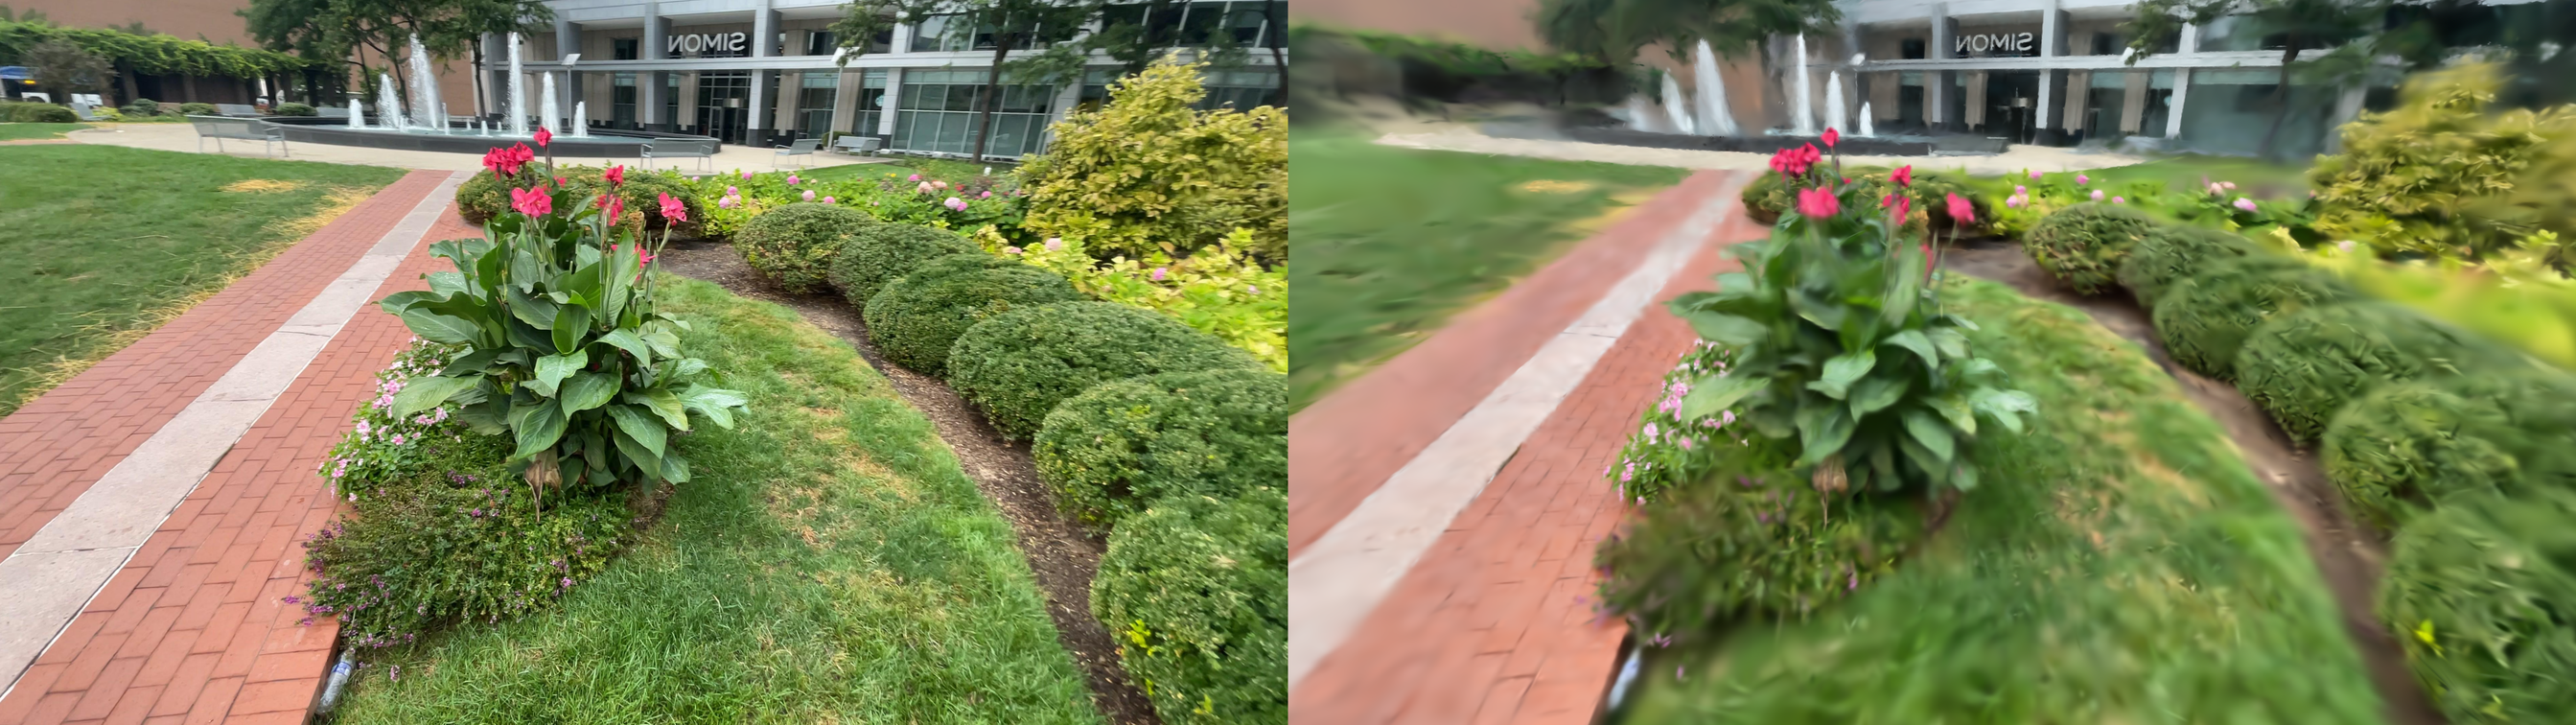
\includegraphics[width=\linewidth]{images/iter1_val_step1999_0010_35.png}
    \caption{Iteration 1}
  \end{minipage}
  \hfill
  \begin{minipage}{0.45\textwidth}
    \centering
    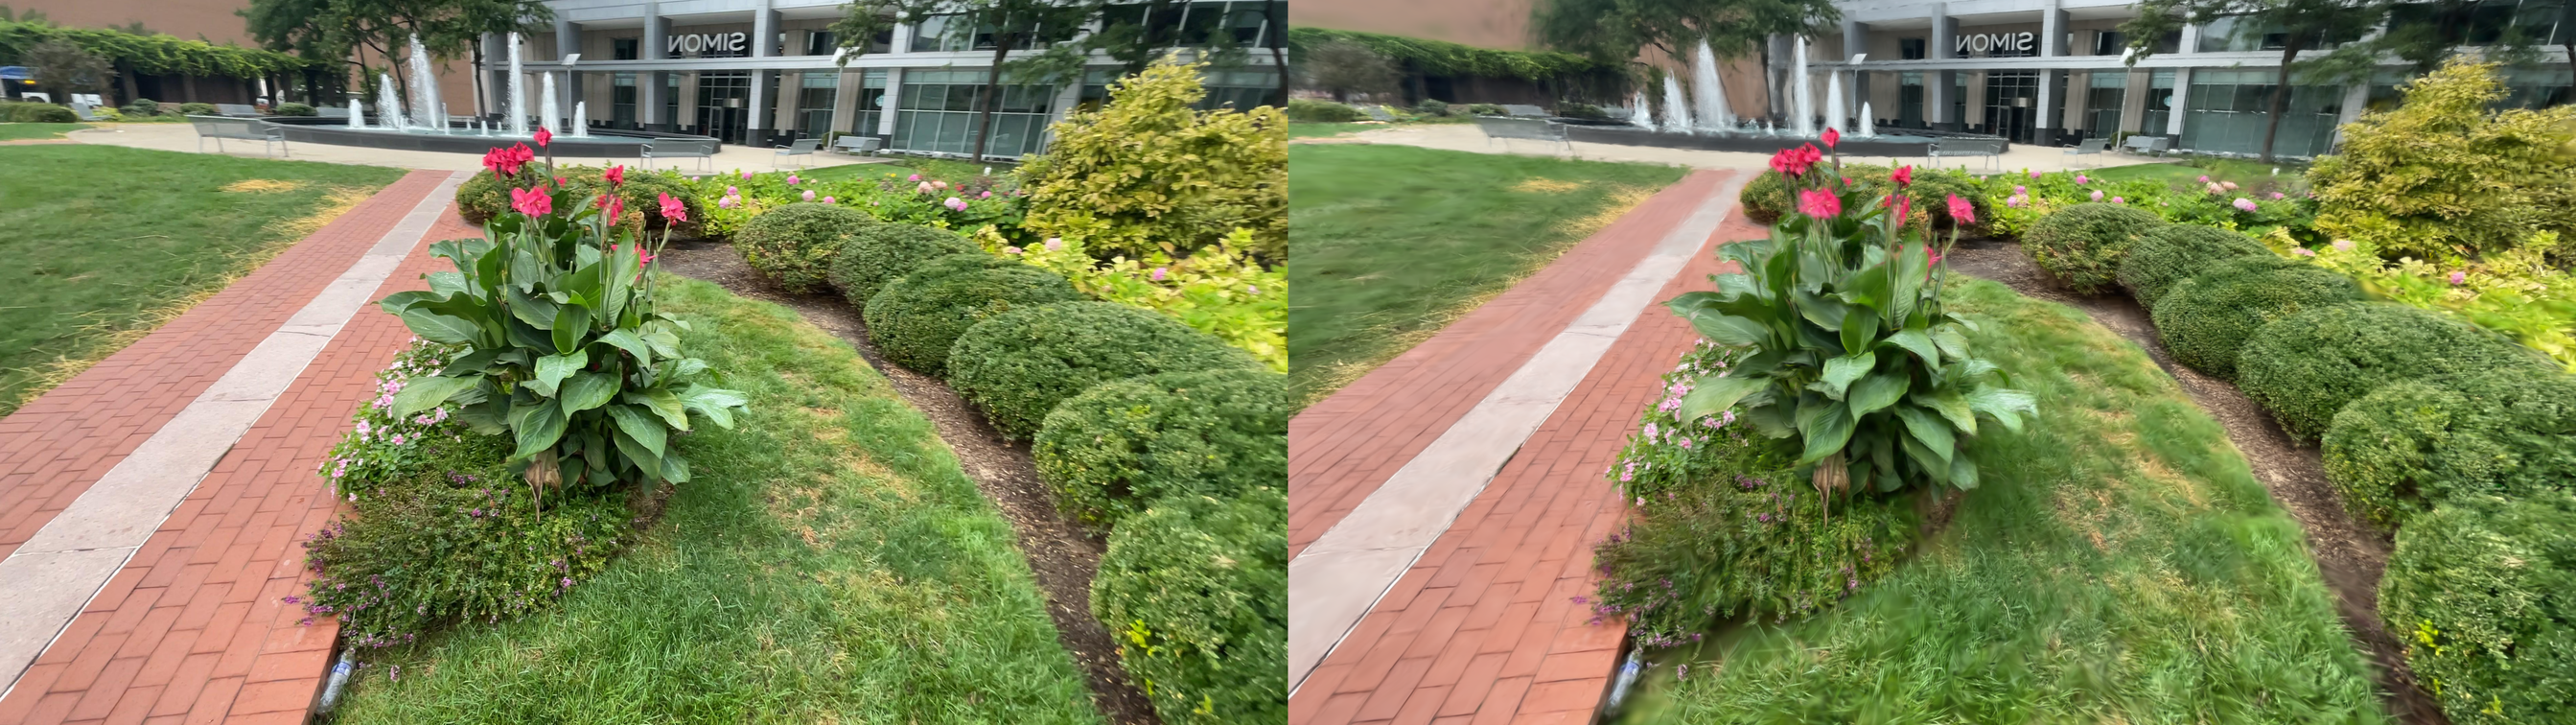
\includegraphics[width=\linewidth]{images/iter2_val_step29999_0010_35.png}
    \caption{Iteration 2}
  \end{minipage}
  \caption{Rasterized views of the Gaussian splatting reconstruction per agentic loop iteration}
  \label{fig:agentic_views}
\end{figure}
\noindent At the end of the first Actor-Critic loop, the Critic agent provided the following feedback to the Actor agent: \\

\noindent\title{Example Critic Agent Feedback:}
\begin{figure}[h]
\centering
\begin{verbatim}
STATUS: REJECTED

CRITIQUE: The rendered viewpoints 
exhibit extreme blurring and a 
complete loss of high-frequency
detail, resulting in critically low PSNR 
and SSIM metrics.

RECOMMENDATION: Increase the number of 
training iterations and adjust 
densification parameters to allow 
for more granular Gaussian refinement 
and detail capture.
\end{verbatim}
\caption{Example Critic Agent Feedback}
\label{fig:critic-agent-prompt}
\end{figure}

\noindent The Actor agent in turn decided to alter the configuration by lowering the density gradient threshold from 0.0002 to 0.0001 and increasing the total training steps from 2,000 to 30,000.\\

\begin{table}[h]
  \centering
  \caption{Training evaluation metrics for the final iteration of Gaussian splatting for each agentic loop}
  \label{tab:training_metrics}
  \begin{tabular}{ccccc}
    \toprule
    \textbf{Iter \#} & \textbf{\# Training Steps} & \textbf{PSNR} & \textbf{SSIM} & \textbf{LPIPS}\\
    \midrule
    1 & 2,000  & 18.593 & 0.5306 & 0.7727 \\
    2 & 30,000 & 19.769 & 0.5802 & 0.4574 \\
    \bottomrule
  \end{tabular}
\end{table}

\begin{table}[h]
  \centering
  \caption{Gaussian splatting training parameters for each agentic loop}
  \label{tab:training_params}
  \begin{tabular}{cccc}
    \toprule
    \textbf{Iter \#} & \textbf{\# Training Steps} & \textbf{\makecell{densify\_grad\\threshold}} & \textbf{\makecell{opacity\_cull\\threshold}} \\
    \midrule
    1 & 2,000  & 0.0002 & 0.05 \\
    2 & 30,000 & 0.0001 & 0.05 \\
    \bottomrule
  \end{tabular}
\end{table}